%% prelim.tex

\section{Preliminaries}
\label{sec:prelim}

\subsection{Texts, substrings, prefixes, and suffixes}
For any integers $i\le j$, we define intervals $[i]=\set{1,\dots,i}$ and $[i, j] = \set{i, i+1, \dots, j}$. Throughout this paper, we assume the word RAM model with machine word size $w = \floor{\log n}$ with input size $n$~\cite{navarro2016cds:book}.

Let $\Sigma = \set{c_1,\dots,c_\sigma}$ be an alphabet of $\sigma \ge 2$ characters. Let us fix a string $S[1..n] = S[1]\dots S[n] \in \Sigma$ of length $n$ over $\Sigma$, called a \textit{text}, delimited by the mutually distinct endmarkers $S[1]=\#$ and $S[n]=\daller$, which do not appear elsewhere in $T$, and are smaller than any other characters. We write $S[p,q]$ for the substring $S[p]S[p+1]\dots S[q]$ with $p\le q$. For any $p$, the substring $S[1,p]$ and $S[p,n]$ are the \textit{prefix} and the \textit{suffix} of $T$, respectively. In what follows, $\Pref(T)$, $\Substr(T)$, and $\Suf(T)$ denote the sets of all prefixes, substrings, and suffixes of $T$, respectively.
%%%
For any string $W$, if $S[p, p+|W|-1] = P$ holds, then we say that $W$ \textit{occurs in $T$ at the start position} $p$ or \textit{the end position} $q = p + |W| - 1$ . We denote by $\spos(W)$ and $\epos(W)$ the sets of all start and end positions of $W$, respectively. The number of occurrences of $W$ in $T$ is denoted by $\occ(W) = |\spos(W)| = |\epos(W)|$. The following monotone property of the occurrences will play a key role in the following sections.  

\begin{lemma}[monotone property]
  \label{lem:occ:monotonicity}
  For any substrings $U, W \in \substr(T)$, we have the following conditions. 
(1) If $U$ is a prefix of $W$ then $\spos(W) \subseteq \spos(U)$ holds, while  
(2) if $U$ is a suffix of $W$ then $\epos(W) \subseteq \epos(U)$ holds. 
\end{lemma}


%% %%%%%%
%% %%%% fig2.tex

\begin{figure}[t]
  \includegraphics[width=\textwidth]{fig/exp1/fwdstree.pdf}
  \caption{{fig/exp1/fwdstree.pdf}}
\end{figure}

\begin{figure}[t]
  \includegraphics[width=\textwidth]{fig/exp1/revstree.pdf}
  \caption{{fig/exp1/revstree.pdf}}
\end{figure}


%% \begin{figure}[p]
%% \centering  
%%   \includegraphics[height=0.45\textwidth]{fig/exp1/fwdstree.pdf}
%%   \subcaption{{fig/exp1/fwdstree.pdf}}
%% %% \end{figure}

%% %% \begin{figure}[t]
%%   \includegraphics[height=0.4\textwidth]{fig/exp1/revstree.pdf}
%%   \subcaption{{fig/exp1/revstree.pdf}}
%% %% \end{figure}

%% %% \begin{figure}[t]
%%   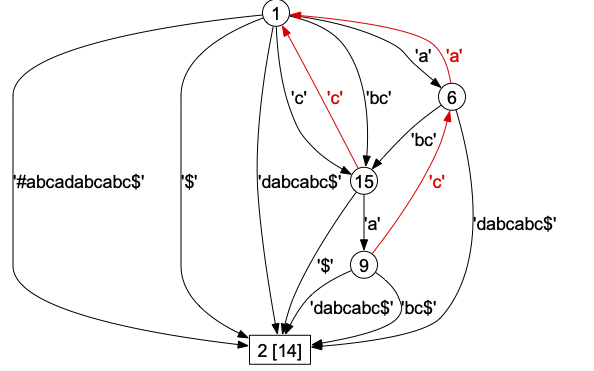
\includegraphics[height=0.45\textwidth]{fig/exp1/cdawg.pdf}
%%   \subcaption{{fig/exp1/revstree.pdf}}
%%   \caption{{fig/exp1/fwdstree.pdf}}
%% \end{figure}
%% %%%%%%

\subsection{Maximal repeats}
\label{sec:mr}
%%%
We introduce the class of maximal repeats (See~Raffinot~\cite{raffinot2001maximal} and Inenaga \textit{et al.}~\cite{inenaga2005line} for details). 
We fix an input text $S[1,n] \in \Sigma^n$ of length $n$.
%%%
Any subword $W$ of $T$ is a \textit{repeat} in $T$ if it occurs at least twice in $T$, namely, $\occ(W) \ge 2$.
A repeat $W$ is said to be \textit{left-branching} (resp.~\textit{right-branching}) in $T$ if either 
(1) $W$ is a prefix  of $T$ (resp.~a suffix of $T$), or 
(2) both of $\occ(aW) \ge 1$ and $\occ(bW) \ge 1$ (resp.~$\occ(Wa) \ge 1$ and $\occ(Wb) \ge 1$) hold for distinct characters $a\not= b$ in $\Sigma$ (including $\#$ and $\daller$). We also refer to left and right branching repeats, respectively, as \textit{left-branching} and \textit{right-branching} repeats. We denote by $\LM(T)$ and $\RM(T)$, respectively, the sets of all left-branching and all right-branching repeats in $T$.

\begin{definition}[maximal repeats, Raffinot~\cite{raffinot2001maximal}]\rm 
  Then, we define a \textit{maximal repeat} of a text $S$ to be any repeat $W$ that is both right-branching and left-branching in $S$. 
\end{definition}


In what follows, we denote by $\M(T)$ the set of all maximal repeats in $S$.
By definition, $\M(T) = \LM(T)\cap\RM(T)$ holds.

For any string $U, W$, we write $U \equiv_L W$ (resp. $U \equiv_R W$) when $\spos(U) = \spos(W)$ (resp. $\epos(U) = \epos(W)$). For any string $W$, the equivalence class with respect to $\equiv_L$ and $\equiv_R$ to which $W$ belongs are denoted by $[W]_L$  and $[W]_R$, respectively. Furthermore, for any substring $W$ of $S$ with $\occ(W) \ge 1$, we denote the \textit{longest elements} of $[W]_L$ and $[W]_R$ by $\rext W$ and $\lext W$, respectively, which are called the \textit{maximal right-extension} (resp.~\textit{maximal left-extension}) of $W$. Then, we define the \textit{maximal extension} of $W$, denoted by $\mext W$ to be the substring 
\begin{align*}
  \mext W = \lext{(\rext{W})} = \rext{(\lext{W})}
\end{align*}
obtained from $W$ by applying operations $\rext\cdot$ and $\lext\cdot$ in any order. We see that the operation $\mext\cdot$ is \textit{idempotent}, i.e., further application of the operator to $\mext W$ does not change itself.
We define the equivalence relation $\equiv$ over $\substr(T)$ as: for any string $U, W$, $U \equiv W \iffdef \mext U = \mext W$. Then, we denote the equivalence class with respect to $\equiv$ by $[W]$. The next lemma is fundamental in our discussion. 

\begin{lemma}
  For any repeat $W$ in a text $S$, 
  (1) $W$ is a maximal repeat in $S$ if and only if 
  (2) there exists a repeat $U$ in $S$ such that $W = \mext U$. 
\end{lemma}

The \textit{compact directed acyclic word graph} (CDAWG) of a text $S$, denoted by $CDAWG(T)$, is a compact data structure proposed by Blumer \textit{et al.}~\cite{blumer1987complete}, which is obtained by merging isomorphic subtrees of the suffix tree of $S$. Formally, the CDAWG for $S$ is defined as follows. 

\begin{definition}[CDAWG]
  For any text $S$, $CDAWG(T)$ is an edge-labeled DAG $C = (V, E)$ such that
  \begin{align*}
    V &= \sete{ \rstate{\rext{U}} \mid U \in \substr(T) },  
    \\
    E &=
    \sete{ (\rstate{\rext U}, a\beta, \rstate{\rext{Ua}})
      \mid U, Ua \in V, a \in \Sigma, \beta \in \Sigma^*,
      \rext{Ua} = Ua\beta, \rext{U} \not= \rext{Ua}
    }, 
  \\
  F &= \sete{ (\rstate{\rext{aU}}, \rstate{\rext{U}})
  \mid aU, U \in \substr(T), a \in \Sigma, 
  %\mext{aU} = \beta a \mext{U}, 
  \rext{aU} \not= \rext{U}
}. 
  \end{align*}
where the nodes $\rstate\eps$ and $\rstate T$ are the initial and final state, respectively, and elements of $E$ and $F$ are called \textit{foward edges} (or \textit{goto edges}) and \textit{backward edges} (or \textit{suffix links}, \textit{Weiner links}), respectively. 
\end{definition}

In \cref{fig:cdawg}, we show an example of a CDAWG.
Raffinot~\cite{raffinot2001maximal} showed that following characterization of $\M(T)$ in terms of the CDAWG. 

\begin{theorem}[Raffinot~\cite{raffinot2001maximal}]
  \label{thm:raffinot:mr:cdawg}
  A substring $W \in \Sigma^+$ is a maximal repeat in $S$ if and only if $W$ is a representative of a branching (or internal) node of the CDAWG of $S$. All substring $U$ with unique occurrences, i.e., $\occ(U) = 1$, are represented by the sink $\rstate{T}$. 
\end{theorem}

From~\cref{thm:raffinot:mr:cdawg}, we can put 
\begin{enumerate*}[(i)]
\item $V \simeq \sete{ \mext{U} \mid U \in \substr(T) }$ and 
\item $E \simeq $ $\sete{ ({\mext W}, a\beta, {\mext{Wa}}) \mid W, Wa \in \substr(T), a \in \Sigma, \beta \in \Sigma^*, \rext{Wa} = Wa\beta, \rext{W} \not= \rext{Wa}}$, and 
\item $F \simeq  \sete{ (\mext{aU}, \beta a, \mext{U}) \mid U, aU \in \substr(T), a \in \Sigma, \mext{aU} = \beta a\mext{U}, \mext{aU} \not= \mext{U}}$. 
\end{enumerate*}
% Now, we define the \textit{suffix links} (or the \textit{Weiner links}) of $CDAWG(T)$ by the links from a node $\mext{aU}$ to its longest suffix $\mext{U}$ different from itself. 
The reverse $W = F^{-1}$ of the suffix links $F$ are called the \textit{Weiner edges} (or \textit{reverse edges}). 
We denote by $e_R = |E|$ and $e_L = |F|$ the numbers of its forward or reverse edges, respectively.

Then, we immediately obtain the next theorem from~\cite{raffinot2001maximal}, which is a start point of our discussion on enumeration of maximal repeats. 

\begin{theorem}[Raffinot~\cite{raffinot2001maximal}]\label{thm:raffinot:mr:enum}
The set $\M(T)$ of all maximal repeats in $S$ can be enumerated in $O(\min\set{e_L, e_R})$ with $CDAWG(T)$ consisting of goto edges and Weiner links. 
\end{theorem}

\begin{proof}
Since $\M(T) \simeq V$ from~\cref{thm:raffinot:mr:cdawg}, it is sufficient to enumerate the node set $V$ of the DFS of $G = CDAWG(T)$. It can be done in $O(e_R)$ time by traversing the forward edges of $E$, or in $O(e_R)$ time by traversing the reverse edges of $E$. By simultaneously running both algorithms alternating them at each step, and taking the shorter one, we obtain $O(\min\set{e_L, e_R})$ time complexity. \qed. 
\end{proof}


%% %%%%%%
%% %% size: n=12
\begin{table}[t]
\caption{
  The set of lexicographically ordered suffixes of a string \texttt{abcadabcabc\daller} of length $n=13$, where $\# < \daller < a < b < c < d$ and the index starts from $0$. 
}
\ttfamily
\centering 
\begin{tabular}{wc{2.5em}wc{2.5em}wc{2.5em}wc{2.5em}lcccc}
%% \hline
\toprule
rank	& SA	& BWT	& LCP		& suffix	\\
\midrule
0	& 0	& \$	& 0		& \#abcadabcabc\$	\\
1	& 12	& c	& 0		& \$	\\
2	& 9	& c	& 0		& abc\$	\\
3	& 6	& d	& 3		& abcabc\$	\\
4	& 1	& \#	& 4		& abcadabcabc\$	\\
5	& 4	& c	& 1		& adabcabc\$	\\
6	& 10	& a	& 0		& bc\$	\\
7	& 7	& a	& 2		& bcabc\$	\\
8	& 2	& a	& 3		& bcadabcabc\$	\\
9	& 11	& b	& 0		& c\$	\\
10	& 8	& b	& 1		& cabc\$	\\
11	& 3	& b	& 2		& cadabcabc\$	\\
12	& 5	& a	& 0		& dabcabc\$	\\
\bottomrule
\end{tabular}
\end{table}


%% size: n=12
\begin{table}[t]
\caption{
  An example of the rank, suffix, inverse suffix, and Burrows-Wheeler Transformation (BWT), and longest common prefix arrays, and the set of lexicographically ordered suffixes of a text \texttt{abcadabcabc\daller} of length $n=13$, where $\# < \daller < a < b < c < d$ and the index starts from $0$. 
}\label{tbl:arrays}
\ttfamily
\centering 
\begin{tabular}{wc{2.5em}wc{2.5em}wc{2.5em}wc{2.5em}lcccc}
%% \hline
\toprule
rank	& SA	& BWT	& LCP		& suffix	\\
\midrule
0	& 0	& \$	& 0		& \#abcadabcabc\$	\\
1	& 12	& c	& 0		& \$	\\
2	& 9	& c	& 0		& abc\$	\\
3	& 6	& d	& 3		& abcabc\$	\\
4	& 1	& \#	& 4		& abcadabcabc\$	\\
5	& 4	& c	& 1		& adabcabc\$	\\
6	& 10	& a	& 0		& bc\$	\\
7	& 7	& a	& 2		& bcabc\$	\\
8	& 2	& a	& 3		& bcadabcabc\$	\\
9	& 11	& b	& 0		& c\$	\\
10	& 8	& b	& 1		& cabc\$	\\
11	& 3	& b	& 2		& cadabcabc\$	\\
12	& 5	& a	& 0		& dabcabc\$	\\
\bottomrule
\end{tabular}
\end{table}
%%%%%%%%%%5


%%% table2.tex : basic text indexing structures
%% table2.tex

%% basic text indexing structures : array-based 
\begin{table}[t]\centering\tabcolsep=.25em
\caption{Array-based text indexing structures for static texts, where
the columns SA, ISA, TA, and LCE indicate the times for accessing the  suffix and the inverse suffix arrays, text $T$, and the LCE query. See \cref{table:summary} for $s_r(n)$  and $s_\delta(n)$. 
}\label{table:arrays}
\medskip
\begin{tabular}{l>{\centering}p{5em}>{\centering}p{7em}cccclll}\toprule
Structure	& Construct\-ion time   & Space (words) & \multicolumn{3}{c}{Query time}	\\
\cmidrule{4-6}
& &  & SA \& ISA	& TA	& LCE	 \\
  \midrule
MM~\cite{manber:myers1993suffixarrays}	& $O(n)$   & $O(n)$	& $O(1)$	& $O(1)$	& $O(1)$	\\
Belazzougui+~\cite{belazzougui2020linear} & $O(n)$   & $O(n\log n/\log\sigma)$	& $O(1)$	& $O(1)$	& $O(1)$	\\
%$s_r(n) = O(r\log(n/r)\log n)$, 
Gagie+~\cite{gagie:navarro:prezza2020fully}	& $s_r(n)$   & $O(r\log(n/r))$	& $O(\log(n/r))$	& $O(\log(n/r))$	& $O(\log(n/r))$	\\
Kempa+~\cite{kempa:kociumaka2023collapsing}	& $s_\delta(n)$   & $O(\delta \log\frac{n\log\sigma}{\delta\log n})$	& $O(\log^{4+\eps} n)$	& $O(\log n)$	& $O(\log n)$	\\
%% na	& sp	& sa	& isa	& ta	& lce	& reference \\
\bottomrule
\end{tabular}
\end{table}
%% EOF


 %% static indexes 
%%%


\subsection{Array-like text indexing data structures}
%%%%%%%%%%5
The \textit{suffix array}~\cite{manber:myers1993suffixarrays} of $S$ is an array $SA[1,n] \in [n]^n$ such that all suffixes of $S$ are ordered as $S[SA[1] < S[SA[2], n] < \dots < S[SA[n], n]$ in the lexicographic order $<$ on suffixes. Each $k \in [n]$ is called the (lexicographic) \textit{rank} of the suffix $S[SA[k], n]$ in $SA$. 
The \textit{inverse suffix array}~\cite{manber:myers1993suffixarrays} is an array $ISA[1,n] \in [n]^n$ defined such that $SA[ISA[p]] = p$ for all positions $p \in [n]$. For any strings $s, t$, we denote by $lcp(s, t)$ the length of the longest common prefix of $s$ and $t$. 

The \textit{longest common prefix (LCP) array}~\cite{manber:myers1993suffixarrays,kasai:lee2001lcp:linear} is an array $LCP[1,n] \in [n]^n$ such that $LCP[1] = 0$ and $LCP[k] = lcp(S[SA[k-1],n], S[SA[k],n])$ for all ranks $k \in [n]$. For any positions $p_1, p_2 \in [n]$ in $S$, we denote the \textit{LCE query} by $\LCE(p_1, p_2) = lcp(S[p_1..n], S[p_2..n])$. 
%For any ranks $k_1, k_2$, the LCE query can be answered using the LCP array with the range minima structure by $\LCE(SA[k_1], SA[k_2]) = \op{RMQ}_{LCP}(k_1+1, k_2) = \min\set{LCP[k] \mid k \in [k_1+1, k_2] }$.
%%% 
The \textit{Burrows-Wheeler Transformation (BWT) array}~\cite{burrows:wheeler1994blocksorting} is an array $BWT[1,n] \in \Sigma^n$ representing the permutation of $S[1,n]$ such that $BWT[k] = \daller$ if $SA[k] = 1$ and $BWT[k] = S[SA[k]-1]$ otherwise for all ranks $k \in [n]$. 
For any rank $k$, we define the \textit{LF-mapping} by $LF(k) = ISA[n]$ if $SA[k]=1$ and $LF(k) = ISA[SA[k]-1]$ otherwise. 

All of these arrays can be constructed in $O(n)$ time from a text $S[1,n]$ (See, e.g.,~\cite{navarro2016cds:book})
%%%
In \cref{tbl:arrays}, we show an example of the above indexing array strucrures for the same text \texttt{abcadabcabc\daller} in the previous example.  

\subsection{Rich representation of a substring}
In our problem, maximal repeats are represented in the concise encoding of substrings of $S$, called the rich representation~\cite{kasai:lee2001lcp:linear,abouelhoda2004replacing,belazzougui2020linear}, which is an extension of the well-known SA-interval~\cite{manber:myers1993suffixarrays}. 

\begin{definition}
The \textit{rich representation} of a substring $W$ of~$S$
%denoted by $\repr(W)$, 
is the triple $\repr(W) = (L(W), R(W), |W|)$ of integers such that
(i) $L(W)$ and $R(W)$ are the left and the right ends 
  \begin{align*}
    L(W) &= \min\sete{ k \in [1..n] \mid SA[k] \in \spos(W)  }
  \\R(W) &= \max\sete{ k \in [1..n] \mid SA[k] \in \spos(W)  }
  \end{align*}
of the contiguous subinterval $\intr(W) = [L(W), R(W)]$ on the suffix array $SA[1,n]$ of $S$ (see~\cite{abouelhoda2004replacing,kasai:lee2001lcp:linear,belazzougui2020linear}), and
(ii) $|W| \ge 0$ is the length of $W$.
\end{definition}

It is shown that $\intr(W) = \spos(W)$. From a rich representation $\tau = (L, R, \ell)$, we can reconstruct the associated substring $W$ such that $\repr(W) = \tau$ by $W = S[SA[k], SA[k]+\ell-1] \in \Sigma^{\ell}$ for any rank $k \in [L,R]$. 
For example, in \cref{tbl:arrays}, the substring $\mathtt{bc}$ has the representation $\repr(W) = (6,8, 2)$ since $W$ has length $2$ and its occurrences of $W$ occupies the interval $[6,8]$ in $SA[0,12]$. 

The \textit{reversed text} is the string $T\rev = S[n]S[n-1]\dots S[1] \in \Sigma^n$ obtained from $S$ by reversing the order of its characters. 
We write $SA\rev$, $ISA\rev$, $LCP\rev$, and $BWT\rev$ for 
the arrays $SA$, $ISA$, $LCP$, and $BWT$ of the reversed text $T\rev$, respectively.

\subsection{Suffix trees}

First, we review the suffix tree of a text $S$~\cite{gusfield1997algorithms} in our terminology.
Formally, the suffix tree for $S$ is defined as follows. 

\begin{definition}[suffix tree]\rm
  \label{def:stree}
  For any text $S$, the suffix tree of $S$, denoted by $\stree(T)$, is an edge-labeled tree $C = (V, E, F)$ such that
  \begin{align*}
    V &= \sete{ \rext{U} \mid U \in \substr(T) },  
    \\
    E &=
    \sete{     (\rext U, a\beta, \rext{Ua})
      \mid \rext{U}, \rext{Ua} \in V, a\in\Sigma, \beta \in \Sigma^*,
      \rext{Ua} = U a\beta 
    }
    % \\
    % E &=
    % \sete{     (\rext U, \beta, U\beta)
    %   \mid U, U\beta \in V, a\in\Sigma, \beta \in \Sigma^+,
    %   \rext{Ua} = U\beta 
    % }
    \\
    F &=
    \sete{ (a\rext{U}, a, \rext{U})
      \mid a\rext{U}, \rext{U} \in V, a\in\Sigma
    }
  \end{align*}
where $\rext\eps \in V$ is the root. Elements of $E$ and $F$ are called \textit{foward edges} (or \textit{goto edges}) and \textit{suffix links}. 
\end{definition}

We let $W = F^{-1}$ to be the set of the inverse links of $F$, where its elements are called \textit{Weiner edges}, and call the edge-labeled tree $(V, W)$ the \textit{Weiner tree} (or the \textit{suffix link tree}) of $S$. 
In \cref{fig:fwdstree}, we show an example of the suffix tree $\stree(T)$ for a text $T = \mathtt{\#abcadabcabc\$}$ of length $n = 13$. In the figure, the circle and boxes indicate the branching nodes and leaves in $V$, respectively. Besides this, black and red arcs indicate the forward and backward edges in~ $E$, respectively. 


%% EOF
